\documentclass{beamer}
\usepackage[T1]{fontenc}
\usepackage[utf8]{inputenc}
\usepackage[ngerman,english,dutch,strings]{babel}
\usepackage{latexsym} 
\usepackage{amsfonts} 
\usepackage{amsmath}
\usepackage{amssymb}
\usepackage{amsthm}
\usepackage{beamerthemesplit}
\usepackage{bbm}

\AtBeginSection[]{
  \begin{frame}
  \vfill
  \centering
  \begin{beamercolorbox}[sep=8pt,center,shadow=true,rounded=true]{title}
    \usebeamerfont{title}\insertsectionhead\par%
  \end{beamercolorbox}
  \vfill
  \end{frame}
}

\title{Binäre Klassifikation mit Python}
\author{Lennart Duvenbeck, Adrian Schoch, Markus Duong}
\date{09.07.2019}

\begin{document}
\maketitle
\begin{frame}{Inhaltsverzeichnis}
  \tableofcontents
\end{frame}

\section{Verfahren und Aufgabenstellung}

\subsection{Verfahren}
\begin{frame}
Gegeben: 
\begin{description}
\item[1.] Trainings-Datensatz D
\item[2.] Test-Datensatz $D^{'}$
\item[3.] eine Menge möglicher k: K
\end{description}
Gesucht: resultierender Klasiifikator: 
\[
f_ {D} := \text{sign} \bigg( \sum_{i=1}^{l} f_{D_{\textbackslash i}, k^{*}}\bigg)
\]
Also: Bestimme das optimale $k^* \in K$
\end{frame}



\begin{frame}
Zerlegen des Datensatzes in l etwa gleichgroße Teildatensätze:
\[
D= D_1 \cup D_2 \cup ... \cup D_l
\]
Definition der "Komplemente":
\[
D_{\textbackslash i} := D_{1} \cup ... \cup D_{i-1} \cup D_{i+1} \cup...\cup D_{l}
\]
\end{frame}


\begin{frame}
Betrachte nun jedes mögliche k:\\
Berechne:
\[ \mathcal{R}_{D_i}(f_{D \textbackslash i ,k})= \frac{1}{m_j} \sum_{j=1}^{m_i} \mathbbm{1}_{y_{j}' \neq f_{D \textbackslash i ,k}(x_{j}')}
\]
Wobei $m_i$ die Anzahl der Punkte in $D_i$ ist und  
\[f_{D \textbackslash i ,k}(x) = \text{sign} \bigg( \sum_{j =1}^{k} y_{i_{j}}\bigg)
\]
Die $y_{i_j}$ sind dabei die Klassifikationen der k nächsten Nachbarn 
$x_{i_1},....,x_{i_k}$ von x in $D \textbackslash i$
\end{frame}

\begin{frame}
Nun erhält man $k^*$: 
\[k^* = \min \limits_{k \in K} \mathcal{R}_{D_i}(f_{D \textbackslash i ,k})
\]
Und der Klassifikator ist:
\[f_ {D} := \text{sign} \bigg( \sum_{i=1}^{l} f_{D_{\textbackslash i}, k^{*}}\bigg)
\]
\end{frame}

\subsection{Aufgabenstellung}
\begin{frame}
Ziel: classify-Funktion\\
Input: name ,Kset , l \\
Output: name.result.csv, Klassifikationsrate $\mathcal{R}_{D'}(f_{D})$ \\
\vspace{20 mm}
\center{\Huge{EFFIZIENT}}
\end{frame}



\section{Implementierung}
\subsection{Punktsuche}
\begin{frame}
In der Aufgabenstellung: KEINE Normvorgabe\\
Sei $ x \in \mathbb{R} ^n:$\\
Möglichkeiten:
\begin{description}
\item[1.] $L^1-Norm$: $\Vert x\Vert _{1}= \sum_{i=1}^n x_i $
\item[2.] $L^2-Norm$:  $\Vert x\Vert _{2}=\sqrt{ \sum_{i=1}^n x_i ^2} $
\item[3.] $L^{\infty}-Norm$:  $\Vert x\Vert _{\infty}= \max(x_1,....,x_n)$
\end{description}
2. Möglichkeit sehr schlecht, da viele Operationen.\\
Noch 1. und 3. Möglichkeit zur Wahl
\end{frame}


\begin{frame}[fragile]
Umsetzung der $L^1-Norm$:
\begin{verbatim}
def nearest_points_naive_l1(x, D, k):
    n = D.shape[0]
    D = D[:, 1:]
    x = x[1:]
    if k > n:
        k = n  
        warnings.warn("Anzahl
        gesuchter nächster Punkte ist größer als
        Anzahl verfügbarer Punkte")
    E = np.sum(np.abs(x - D), 1)
    I = np.argsort(E)
    return I[:k]
\end{verbatim}
\end{frame}


\begin{frame}[fragile]
Umsetzung der $L^{\infty}-Norm$:
\begin{verbatim}
def nearest_points_naive_sup(x, D, k):
    n = D.shape[0]
    D = D[:, 1:]
    x = x[1:]
    if k > n:
        k = n 
        warnings.warn("Anzahl
        gesuchter nächster Punkte ist größer als 
        Anzahl verfügbarer Punkte")
    E = np.max(np.abs(x - D), 1)
    I = np.argsort(E)
    return I[:k]
\end{verbatim}
\end{frame}

\begin{frame}
Laufzeitmessung durch Einteilung des Datensatzes in die Teildatensätze $D_i$ und  $D_{\textbackslash i}$ für i=1,...,5.\\
Suche für jedes x aus $D_i$ die 200 nächsten Nachbarn aus $D_{\textbackslash i}$.\\
1. Datensatz: "toy-2d.train.csv" (10499 2D-Punkte)\\
2. Datensatz: "toy-4d.train.csv" (10499 10D-Punkte)\\
3. Datensatz: "toy-10d.train.csv" (10499 10D-Punkte)
\end{frame}


\begin{frame}[fragile]
1. Datensatz: "toy-2d.train.csv".\\
\vspace{5mm}
Mit $L^1-Norm$
\begin{verbatim}
6.8030703068 seconds
\end{verbatim}
Mit $L^{\infty}-Norm$
\begin{verbatim}
5.9372479916 seconds
\end{verbatim}
Bei anderen 2D-Datensätzen ähnliche Ergebnisse
\end{frame}


\begin{frame}[fragile]
2. Datensatz: "toy-4d.train.csv".\\
\vspace{5mm}
Mit $L^1-Norm$
\begin{verbatim}
7.5119700432 seconds
\end{verbatim}
Mit $L^{\infty}-Norm$
\begin{verbatim}
8.3533186913 seconds
\end{verbatim}
Bei anderen 4D-Datensätzen ähnliche Ergebnisse
\end{frame}

\begin{frame}[fragile]
3. Datensatz: "toy-10d.train.csv".\\
\vspace{5mm}
Mit $L^1-Norm$
\begin{verbatim}
8.1387059689 seconds
\end{verbatim}
Mit $L^{\infty}-Norm$
\begin{verbatim}
9.7477006912 seconds
\end{verbatim}
\end{frame}
\subsection{erstes lauffähiges Programm}

\subsection{effizienteres Programm}



\section{Interessanter Zwischenergebnisse und ihre graphische Darstellung}
\begin{figure}[h]
\centering
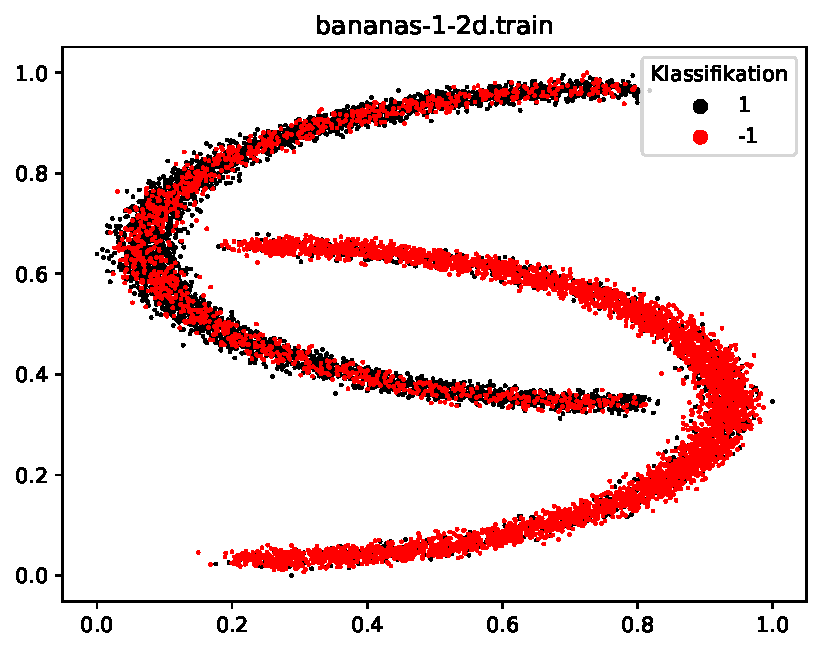
\includegraphics[scale=0.7]{bananas-1-2d-train.pdf}
\label{bananas}
\end{figure}

\begin{figure}[h]
\centering
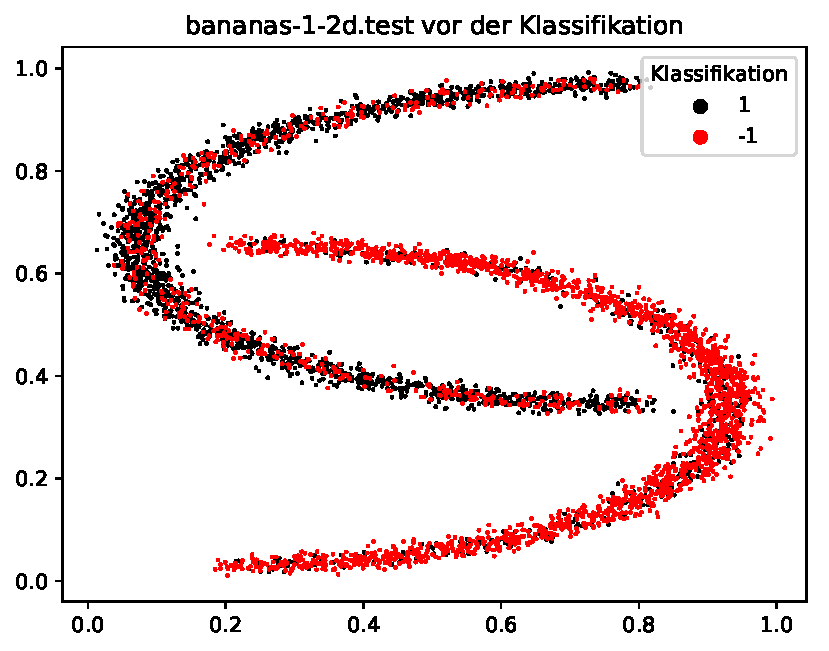
\includegraphics[scale=0.7]{bananas-1-2d-test-vorher.pdf}
\label{bananas}
\end{figure}


\begin{figure}[h]
\centering
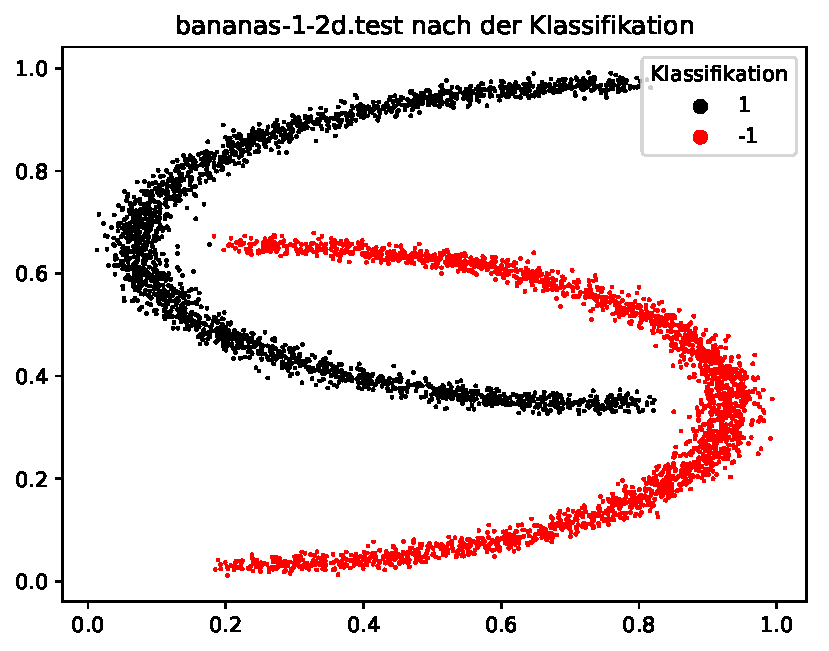
\includegraphics[scale=0.7]{bananas-1-2d-test-nacher.pdf}
\label{bananas}
\end{figure}
\end{document}

